% Chapter 10, Section 5

\section{Sequence-to-Sequence Models \difficultyInline{intermediate}}
\label{sec:seq2seq}

\subsection*{Intuition}

Encoder–decoder models compress a source sequence into a representation and then generate a target sequence step-by-step. Attention augments this by letting the decoder look back at encoder states as needed, creating a dynamic context per output token \cite{Cho2014,Bahdanau2014}.

\subsection*{Historical Context}

Early seq2seq relied on fixed context vectors, which degraded on long inputs. Content-based attention \cite{Bahdanau2014} lifted this bottleneck and paved the way toward Transformer architectures \cite{Vaswani2017}.

% Index and glossary
\index{sequence-to-sequence}
\glsadd{attention-mechanism}

\subsection{Encoder-Decoder Architecture}

The encoder-decoder architecture revolutionized sequence-to-sequence learning by solving a fundamental challenge: how to transform variable-length input sequences into variable-length output sequences of potentially different lengths. Traditional approaches struggled with this asymmetry, as they required fixed input-output dimensions or relied on hand-crafted features that couldn't capture the complex relationships between source and target sequences. The key insight behind this architecture lies in its elegant separation of concerns: the encoder compresses the entire input sequence into a rich, fixed-size representation that captures all essential information, while the decoder uses this representation to generate the output sequence step-by-step, maintaining the temporal dependencies crucial for coherent generation. This design was revolutionary compared to previous architectures because it eliminated the need for explicit alignment between input and output positions, allowing the model to learn implicit correspondences through end-to-end training. Unlike rule-based systems or traditional statistical methods that required extensive linguistic knowledge, the encoder-decoder framework could automatically discover complex mappings between any two sequence domains, making it the foundation for modern neural machine translation and countless other sequence transduction tasks.

For sequence transduction tasks like machine translation \cite{Cho2014,Bahdanau2014}:

\textbf{Encoder:} Processes input sequence into representation (fixed or per-step states)
\begin{equation}
\vect{c} = f(\vect{x}_1, \vect{x}_2, \ldots, \vect{x}_T)
\end{equation}

\textbf{Decoder:} Generates output sequence from representation
\paragraph{Visual aid.} A minimal encoder–decoder with context vector.
\begin{figure}[h]
    \centering
    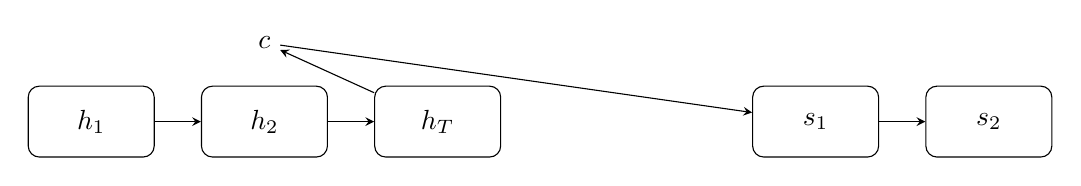
\begin{tikzpicture}[>=stealth, node distance=2.2cm]
        \tikzstyle{enc}=[draw, rounded corners, minimum width=1.6cm, minimum height=0.9cm]
        \tikzstyle{dec}=[draw, rounded corners, minimum width=1.6cm, minimum height=0.9cm]
        \node[enc] (e1) {$\vect{h}_1$};
        \node[enc, right of=e1] (e2) {$\vect{h}_2$};
        \node[enc, right of=e2] (eT) {$\vect{h}_T$};
        \node[above of=e2, yshift=-1.2cm] (c) {$\vect{c}$};
        \draw[->] (e1) -- (e2);
        \draw[->] (e2) -- (eT);
        \draw[->] (eT) -- (c);
        \node[dec, right of=eT, xshift=2.6cm] (d1) {$\vect{s}_1$};
        \node[dec, right of=d1] (d2) {$\vect{s}_2$};
        \draw[->] (c) -- (d1);
        \draw[->] (d1) -- (d2);
    \end{tikzpicture}
    \caption{Encoder–decoder with fixed context vector $\vect{c}$. Attention uses step-dependent $\vect{c}_t$.}
\end{figure}

\begin{equation}
\vect{y}_t = g(\vect{y}_{t-1}, \vect{c}, \vect{s}_{t-1})
\end{equation}

\subsection{Attention Mechanism}

Attention represents one of the most crucial breakthroughs in deep learning, so fundamental that the seminal paper "Attention Is All You Need" \cite{Vaswani2017} demonstrated that attention mechanisms alone could replace entire architectural components like recurrent layers. This paradigm shift occurred because attention solves the fundamental information bottleneck problem in sequence-to-sequence models, where standard approaches compress entire input sequences into a single fixed vector $\vect{c}$, inevitably losing critical information and context. The attention mechanism elegantly addresses this limitation by allowing the decoder to dynamically focus on different parts of the input sequence at each generation step, creating a flexible and context-aware representation that adapts to the specific requirements of each output token.

\textbf{Attention} allows the decoder to focus on relevant input parts by computing a content-based weighted average of encoder states \cite{Bahdanau2014}. At each decoding step $t$:

\begin{align}
e_{ti} &= a(\vect{s}_{t-1}, \vect{h}_i) \quad \text{(alignment scores)} \\
\alpha_{ti} &= \frac{\exp(e_{ti})}{\sum_j \exp(e_{tj})} \quad \text{(attention weights)} \\
\vect{c}_t &= \sum_i \alpha_{ti} \vect{h}_i \quad \text{(context vector)}
\end{align}
Common scoring functions $a(\cdot)$ include additive (Bahdanau) attention using a small MLP, and multiplicative/dot-product attention which is parameter-efficient and forms the basis for scaled dot-product attention in Transformers \cite{Vaswani2017}. Attention weights $\alpha_{ti}$ are interpretable as soft alignments between target position $t$ and source position $i$ (see \cite{WebAttentionWikipedia}). For a broader overview, consult standard references \cite{WebDLBRNN,D2LChapterAttention}.

\paragraph{Training and inference.} Attention is trained end-to-end with the seq2seq objective. During inference, attention enables the model to retrieve the most relevant encoder features for each generated token, improving long-input performance and handling reordering. Variants include multi-head attention, local/monotonic attention for streaming, and coverage terms to reduce repetition.

Benefits:

\textbf{Dynamic context for each output:} Unlike traditional approaches that use a single, static context vector for all output positions, attention creates a unique, dynamically computed context vector for each decoding step. This means that when generating the word "cat" in a translation, the model can focus on the relevant source words like "gato" or "chat," while when generating "dog," it shifts its attention to "perro" or "chien." This adaptive context selection allows the model to maintain fine-grained relationships between source and target elements, dramatically improving translation quality and coherence across different linguistic structures.

\textbf{Better for long sequences:} Traditional encoder-decoder models suffer from severe performance degradation on long sequences because the fixed-size context vector becomes an information bottleneck, unable to preserve all the nuanced details from lengthy inputs. Attention mechanisms solve this by providing direct access to all encoder states, allowing the model to selectively retrieve relevant information regardless of sequence length. This capability is particularly crucial for tasks like document summarization or translating lengthy articles, where the model must maintain awareness of information from the beginning of the document even when generating the final sentences.

\textbf{Interpretable (visualize attention weights):} One of the most remarkable aspects of attention mechanisms is their inherent interpretability, as the attention weights $\alpha_{ti}$ provide a clear, visual representation of which input positions the model considers most relevant for each output token. Researchers can visualize these attention patterns as heatmaps, revealing fascinating insights about how the model learns linguistic alignments, syntactic structures, and semantic relationships. This interpretability has proven invaluable for debugging model behavior, understanding translation errors, and even discovering novel linguistic patterns that the model has learned autonomously, making attention not just a powerful computational tool but also a window into the model's decision-making process.

\subsection{Applications}

\textbf{Machine translation (NMT):} Modern neural machine translation systems power real-time communication across language barriers, enabling instant translation of web pages, documents, and conversations in applications like Google Translate and Microsoft Translator. These systems handle complex linguistic phenomena such as idiomatic expressions, cultural references, and context-dependent meanings that traditional rule-based systems struggled with, making global communication seamless for billions of users worldwide.

\textbf{Text summarization (extractive and abstractive):} News organizations and content platforms rely on sequence-to-sequence models to automatically generate concise summaries of lengthy articles, research papers, and legal documents, helping readers quickly grasp key information without reading entire texts. Financial institutions use these systems to summarize market reports and regulatory documents, while healthcare organizations employ them to distill complex medical literature into actionable insights for practitioners.

\textbf{Question answering and dialogue systems:} Virtual assistants like Siri, Alexa, and Google Assistant leverage sequence-to-sequence architectures to understand user queries and generate natural, contextually appropriate responses across diverse topics and conversation styles. Customer service chatbots powered by these models can handle complex inquiries, maintain conversation context across multiple turns, and provide personalized assistance while reducing human workload and improving response times.

\textbf{Image captioning (CNN/ViT encoder, RNN/Transformer decoder):} Social media platforms and accessibility tools use image captioning to automatically generate descriptive text for photos, helping visually impaired users understand visual content and improving content discoverability through search. Medical imaging systems employ these models to generate detailed reports from X-rays and MRI scans, while autonomous vehicles use them to describe road conditions and potential hazards for safety systems.

\textbf{Speech recognition and speech translation:} Real-time meeting transcription services like Otter.ai and Zoom's live transcription feature use sequence-to-sequence models to convert spoken language into accurate text, enabling accessibility and note-taking for millions of users. Simultaneous interpretation systems at international conferences and diplomatic meetings leverage these technologies to provide real-time translation between speakers of different languages, breaking down communication barriers in global settings.

\textbf{OCR and handwriting recognition:} Banking and financial institutions use OCR systems to automatically process handwritten checks, forms, and documents, dramatically reducing manual data entry and processing time while minimizing human errors. Educational platforms employ handwriting recognition to digitize student notes and assignments, enabling digital archiving, search, and analysis of handwritten content across academic institutions.

\textbf{Code generation and program repair:} Software development platforms like GitHub Copilot and Tabnine use sequence-to-sequence models to suggest code completions, generate functions from natural language descriptions, and automatically fix bugs in existing codebases. These systems help developers write code faster, catch potential errors early, and learn new programming patterns, while automated program repair tools can identify and fix security vulnerabilities and performance issues in large-scale software projects.

